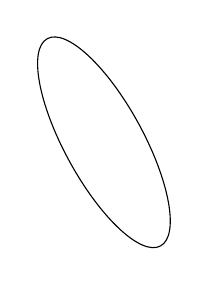
\begin{tikzpicture}
     \draw[rotate=deg(0.5)] (0, 0) ellipse (0.5cm and 1.5cm);
\end{tikzpicture}





%
%
%\documentclass{article}
%\usepackage{pgfplots}
%\usepackage{datatool}
%\DTLloaddb[noheader=false]{coordinates}{data.csv}
%\pgfplotsset{compat=1.12}

%\usepackage{filecontents}

%
%\DTLloaddb[noheader=false]{coordinates}{testdata.csv}
%
%\begin{tikzpicture}	
%
%	\draw[
%	%	rotate=deg(\an),
%	color=orange,very thick] (0,0) ellipse [x radius=2,y radius=1,rotate around={deg(10):(0,0)}];
%
%
%%	\draw [help lines] (-2, -2) grid (2, 2);
%		\draw[step=1,help lines,black!20] (-0.95,-0.95) grid (4.95,4.95);
%		
%	
%	\begin{loopTabbedCsv}{coordinates}{\xc=xc, \yc=yc,\xr=xer,\yr=yer,\an=phi}
%
%	\draw[
%	%	rotate=deg(\an),
%		color=blue,very thick] (\xc, \yc) ellipse [x radius=\xr,y radius=\yr,rotate around={deg(\an):(\xc,\yc)}];
%
%
%	\end{loopTabbedCsv}
%
%%\end{axis}
%
%
%\end{tikzpicture}\\
%



\newcommand\plot[3]{
	\begin{tikzpicture}
	
	% help lines
	\draw[step=1,help lines,black!20] (-0.95,-0.95) grid (4.95,4.95);
	% axis
	\draw[thick,->] (-10,0) -- (10,0);
	\draw[thick,->] (0,-10) -- (0,10);
	
	% points
	\foreach \Point/\PointLabel in {#1}
	\draw[fill=green] \Point circle (0.05) node[above right] {$\PointLabel$};
	
	
	
%	\begin{scope}[xshift=1cm, yshift=2.075]
	
	\foreach \Point/\PointLabel in {#2}
	\draw[fill=red] \Point circle (0.05) node[above right] {$\PointLabel$};

%	\end{scope}
	

	
	#3	
	
	\end{tikzpicture}
	}


\plot{
		(1,2.3)/P0,(2.3,0.5)/P1,(3,2)/P2,(2.5,4.5)/P3
	}{
%		(0.07,1.2)/P0,(1.82,-0.17)/P1,(0.29,-0.81)/P2,(-2.19,-0.21)/P3
(-0.07,1.2)/P0,(-1.82,-0.17)/P1,(-0.29,-0.81)/P2,(2.19,-0.21)/P3
	}{
	\draw[->, thick, blue] 
%(2.2,2.325) -- (2.09100654418751,-0.39852149590928)
(2.2,2.325) -- (2.30899345581249,5.04852149590928)
	node[above right]{1};
	
	\draw[->, thick, orange] 
(2.2,2.325) -- (1.4771135144198,2.35392941962892)
	node[above right]{2};
	}


\plot{
(1,2.3)/P0,(-1,0.5)/P1,(3,2)/P2,(5,3.5)/P3
}{
(-0.82,0.62)/P0,(-3.38,-0.21)/P1,(0.88,-0.48)/P2,(3.32,0.07)/P3
}{
	\draw[->, thick, blue] 
	(2,2.075) -- (9.26955486324896,5.34430729026665)
	node[above right]{1};
	
	\draw[->, thick, orange] 
	(2,2.075) -- (1.91046489706353,2.27408815085112)
	node[above right]{2};
	
}



\begin{tikzpicture}

%	\def\Xmin{0}
%	\def\Ymin{-0.5}

	\begin{axis}[
%	xmin=\Xmin,
%	ymin=\Ymin,
	xmax=50,ymax=50,
	xmin=-50,ymin=-50,
%	domain=-50:50
	]

%	\addplot table [x=xc, y=yc, col sep=comma, only marks, mark=0] {testdata.csv};
%	

%	\draw[red] (-2,1.5) node[anchor=south] {.};


	\addplot table [x=xc, y=yc, col sep=comma, only marks, mark=0] {testdata.csv};
	
	
%	\draw[red] (1,2.3) node {.}
	
%	,{2.3,0.5},{3,2},{2.5,4.5}

%	\begin{loopTabbedCsv}{coordinates}{\xc=xc, \yc=yc,\xr=xer,\yr=yer,\an=phi}
%	
%	%	\draw[rotate=deg(\an)] (\xc, \yc) ellipse (0.5cm and 1.5cm);	
%	%	%		\draw[rotate=deg(\an)] (0, 0) ellipse (0.5cm and 1.5cm);	
%	%	%
%	%	
%	%	\filldraw[blue,fill opacity=0.2] (axis cs:\xc,\yc) ellipse;
%	
%%	(\xc,\yc)
%
%		\filldraw[blue,fill opacity=0.2] (axis cs:2,2) ellipse (0.5cm and 1.5cm);
%
%	
%	\end{loopTabbedCsv}



%	\pgfplotsextra{\DTLforeach*{coordinates}{\x=xc, \y=yc,\xr=xer,\yr=yer,\an=phi}{
%			%x-coor ellipse center, y-coor ellipse center, x-radius of ellipse, y-radius of ellipse, rotation angle of ellipse
%%			\filldraw[blue,fill opacity=0.2] 
%%			(axis cs:\x,\y) ellipse [x radius=\xr,y radius=\yr,rotate around={deg(\an):(\Xmin,\Ymin)}];
%		}
%	}
	
	
	\end{axis}
\end{tikzpicture}